\section{Appendix (6)}
\label{Appendix (6)}
\subsection{Talteori (1)}
\subsubsection{Induktionsprincippet}
At mængden $\N$ har en \nameref{Velordning} vil sige at det har et første
element, hvilket vil sige $\exists s : s \leq x$ for alle $x \in \N$. Dette er
ækvivalent til matematisk induktion der siger:

Lad $P(n)$ være et udsagn hvor der for alle $n \geq 1$ gælder
\begin{enumerate}[(i)]
  \item $P(1)$ er sand.
  \item $P(n)$ er sand $\Rightarrow$ at $P(n + 1)$ er sand.
\end{enumerate}
så kan vi konkludere at $P(n)$ er sand for alle $n \geq 1$.

\subsubsection{Reference (1.1)}
Der gælder $1 + 2 + \cdots + n = \frac{n(n+1)}{2}$

\subsubsection{Grupper (2)}
\label{Grupper (2)}
\subsubsection{Veldefineret}
\label{Veldefineret}
En afbildning $f: X \to Y$ kaldes veldefineret hvis den afbilder alle elementer
i domænet $X$ til et element i codomænet $Y$.

\textit{Uanset valget af repræsentanter for sideklasser så afbilder de til
samme element}.

\subsubsection{Injektiv}
\label{Injektiv}
En afbildning $f: X \to Y$ kaldes injektiv hvis der gælder
\begin{equation*}
  \forall a, b \in X \Rightarrow \text{ hvis } f(a) = f(b), \text{ så er } a
  = b
\end{equation*}
\textit{Alle elementer i domænet X afbilder til et unikt element i Y
$\Rightarrow \mid X\mid \leq \mid Y\mid$}.

\subsubsection{Surjektiv}
\label{Surjektiv}
En afbildning $f: X \to Y$ kaldes surjektiv hvis der gælder
\begin{equation*}
  \forall y \in Y \exists x \in X, \text{ hvor } f(x) = y
\end{equation*}
\textit{Alle elementer i codomænet Y bliver ramt af et element i X $\Rightarrow
\mid X \mid \geq \mid Y\mid$}.

\subsubsection{Bijektiv}
\label{Bijektiv}
En afbildning $f: X \to Y$ kaldes bijektiv hvis den er både
\begin{enumerate}[(i)]
  \item \nameref{Injektiv}. \textit{Alle elementer i codomænet Y bliver ramt af
  et element i X $\Rightarrow \mid X\mid \geq \mid Y\mid$}.  
  \item \nameref{Surjektiv}. \textit{Alle elementer i domænet X afbilder til et
  unikt element i Y $\Rightarrow \mid X\mid \leq \mid Y\mid$}.
\end{enumerate}
\textit{Enhver afbildning der har en invers er bijektiv}

\subsubsection{\textit{Ker(f)}}
\label{Ker(f)}
Lad $f: G \rightarrow K$ være en \nameref{Gruppehomomorfi}, så er:
\begin{equation*}
  Ker(f) = \myset{g \in G \mid f(g) = e}
\end{equation*}
\textit{Kernen af f er mængden af alle elementer i G, som f afbilder til det
neutrale element i K}.

\subsubsection{\textit{f(G)}}
Lad $f: G \rightarrow K$ være en \nameref{Gruppehomomorfi}, så er:
\label{f(G)}
\begin{equation*}
  f(G) = \{f(g) \mid g \in G\} \subseteq K
\end{equation*}
\textit{Billedet af f er alle de elementer i K som f afbilder til fra G}.

\begin{figure}
\begin{center}
  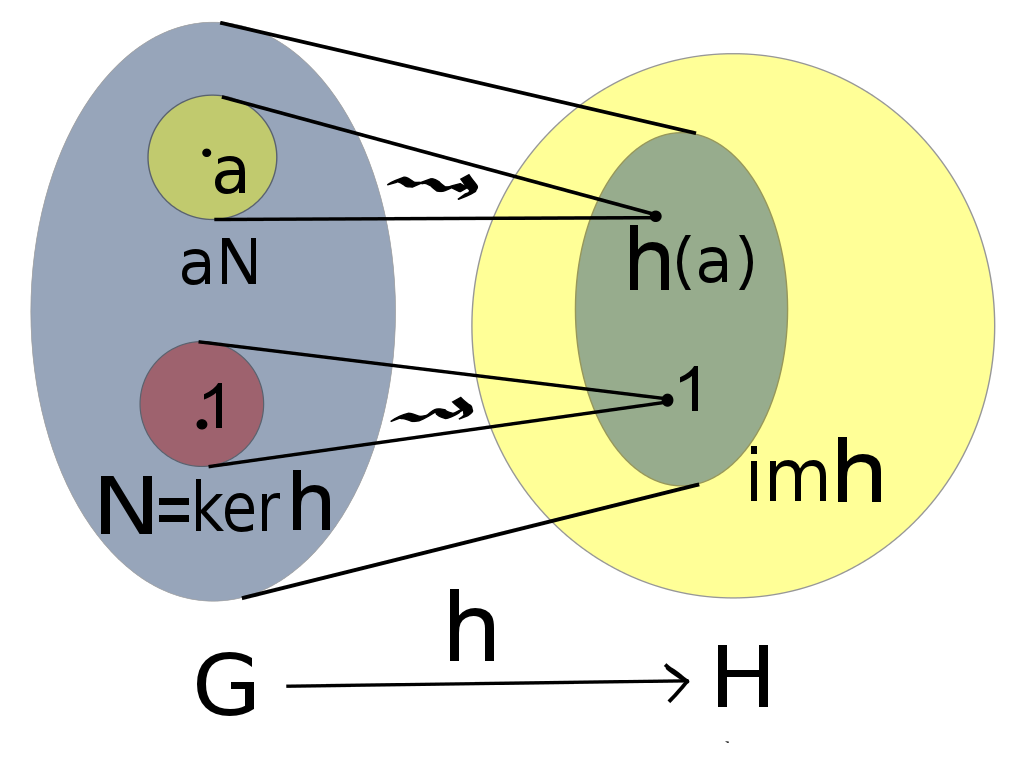
\includegraphics[width=0.8\textwidth]{img/group_homomorphism}
  \caption[labelInTOC]{
  Animation af en gruppehomomorfi $h: G \rightarrow H$. Den lille oval inde i
  $H$ er billedet af $H$. $N$ er kernen af $H$ og $aN$ er en sideklasse til
  $N$.}
  \label{figureLabel}
\end{center}
\end{figure}

\subsection{Gröbnerbaser (5)}
\label{Gröbnerbaser (5)}
\subsubsection{Relation}
\label{Relation}
Def. A.1.1: En relation $R$ på en mængde $S$ er en delmængde $R \subseteq S
\times S$. Vi skriver $xRy$ hvor vi mener $(x,y) \in R$.

\subsubsection{Ækvivalensrelation}
\label{Aekvivalensrelation}
Def. A.1.2: En \nameref{Relation} $R$ på en mængde $S$ er kaldes en
ækvivalensrelation hvis den er
\begin{enumerate}[(i)]
  \item Refleksiv: $xRx \quad \forall x \in S$.
  \item Symmetrisk: $xRy \Rightarrow yRx \quad \forall x,y \in S$.
  \item Transativ: $xRy \myand yRz \Rightarrow xRz \quad \forall x,y,z \in S$.
\end{enumerate}
som eksempel er kongruens modulo et ideal, $I$ en ækvivalensrelation
\begin{equation*}
  x \mycong{y}{I} \iff x - y \in I
\end{equation*}
Dette er det generelle tilfælde af relationen kongruens modulo et heltal i
$\Z$, hvilket også er en ækvivalensrelation.

\subsubsection{Partiel ordning}
\label{Partiel ordning}
Def. A.1.2: En \nameref{Relation} $R$ på en mængde $S$ er kaldes en partiel
ordning hvis den er
\begin{enumerate}[(i)]
  \item Refleksiv: $xRx \quad \forall x \in S$.
  \item Antisymmetrisk: $xRy \myand yRx \Rightarrow x = y \quad \forall x,y
  \in S$.
  \item Transativ: $xRy \myand yRz \Rightarrow xRz \quad \forall x,y,z \in S$.
\end{enumerate}
Som eksempel er $\leq$ en partiel ordning på $\Z$.

\subsubsection{Minimalt element}
\label{Minimalt element}
Et element $s \in S$ med en \nameref{Partiel ordning} $\leq$ siges at være et
minimalt element hvis
\begin{equation*}
  x \leq s \Rightarrow x = s
\end{equation*}
$\forall x \in S$.

\subsubsection{Første element}
\label{Foerste element}
Et element $t \in S$ med en \nameref{Partiel ordning} $\leq$ siges at være
et første element hvis
\begin{equation*}
  t \leq x
\end{equation*}
$\forall x \in S$. Fordi $\leq$ er antisymmetrisk må dette $t$ være unikt. Er
første element er et \nameref{Minimalt element}.

\subsubsection{Total ordning}
\label{Total ordning}
Def. A.3.4: En \nameref{Partiel ordning} $\leq$ på en mængde $S$ kaldes en total
ordning hvis
\begin{equation*}
  x \leq y \myor y \leq x \quad \forall x,y \in S
\end{equation*}

\subsubsection{Velordning}
\label{Velordning}
Def. A.3.5: En \nameref{Partiel ordning} $\leq$ på en mængde $S$ kaldes en
velordning hvis ethver ikke-tomt delmængde $M \subseteq S$ har et
\nameref{Foerste element}.

\subsection{$\langle f_1, \ldots, f_m \rangle$}
\label{f_1..f_m}
\begin{align*}
  &\langle f_1, \ldots, f_m \rangle =\\
  &\myset{a_1(X_1,\ldots,X_m)f_1 + \cdots + a_m(X_1,\ldots,X_m)f_m \mid
  a_1(X_1,\ldots,X_m), b_1(X_1,\ldots,X_m) \in R[X_1,\ldots,X_n]}
\end{align*}
hvilket vil sige alle ``lineære'' kombinationer af $f_1, \ldots, f_m$.